\section{R\'ESUM\'E CONSOLID\'E PUBLIC}
\label{sec:resume}

\ANRinfo{Ce résumé est destiné à être diffusé auprès d’un large public pour promouvoir les résultats du projet, il ne fera donc pas mention de résultats confidentiels et utilisera un vocabulaire adapté mais n’excluant pas les termes techniques. Il en sera fourni une version française et une version en anglais. Il est nécessaire de respecter les instructions ci-dessous.}

\subsection{Résumé consolidé public en français}
Multi-modAl Earth obServaTion Image Analysis 

\ANRinfo{Titre 1 : situe l’objectif  général du projet et sa problématique (150 caractères max espaces compris)}


\ANRinfo{Paragraphe 1 : (environ 1200 caractères espaces compris)
Le paragraphe 1 précise les enjeux et objectifs du projet : indiquez le contexte, l’objectif général, les problèmes traités, les solutions recherchées, les perspectives et les retombées au niveau technique ou/et sociétal}

\subsubsection*{Titre 2 : précise les méthodes ou technologies utilisées (150 caractères max espaces compris)}

\ANRinfo{Le paragraphe 2 indique comment les résultats attendus sont obtenus grâce à certaines méthodes ou/et technologies. Les technologies utilisées ou/et les méthodes permettant de surmonter les verrous sont explicitées (il faut éviter le jargon scientifique, les acronymes ou les abréviations).}


\subsubsection*{Résultats majeurs du projet (environ 600 caractères espaces compris)}

\ANRinfo{Faits marquants diffusables en direction du grand public, expliciter les applications ou/et les usages rendus possibles, quelles sont les pistes de recherche ou/et de développement originales, éventuellement non prévues au départ.\\
Préciser aussi toute autre retombée= partenariats internationaux, nouveaux débouchés, nouveaux contrats, start-up, synergies de recherche, pôles de compétitivité, etc.}


\subsubsection*{Production scientifique et brevets depuis le début du projet}(environ 500 caractères espaces compris) \\
\ANRinfo{Ne pas mettre une simple liste mais faire quelques commentaires. Vous pouvez aussi indiquer les actions de normalisation}


\subsubsection*{Illustration}
\begin{figure}[h]
    \centering
    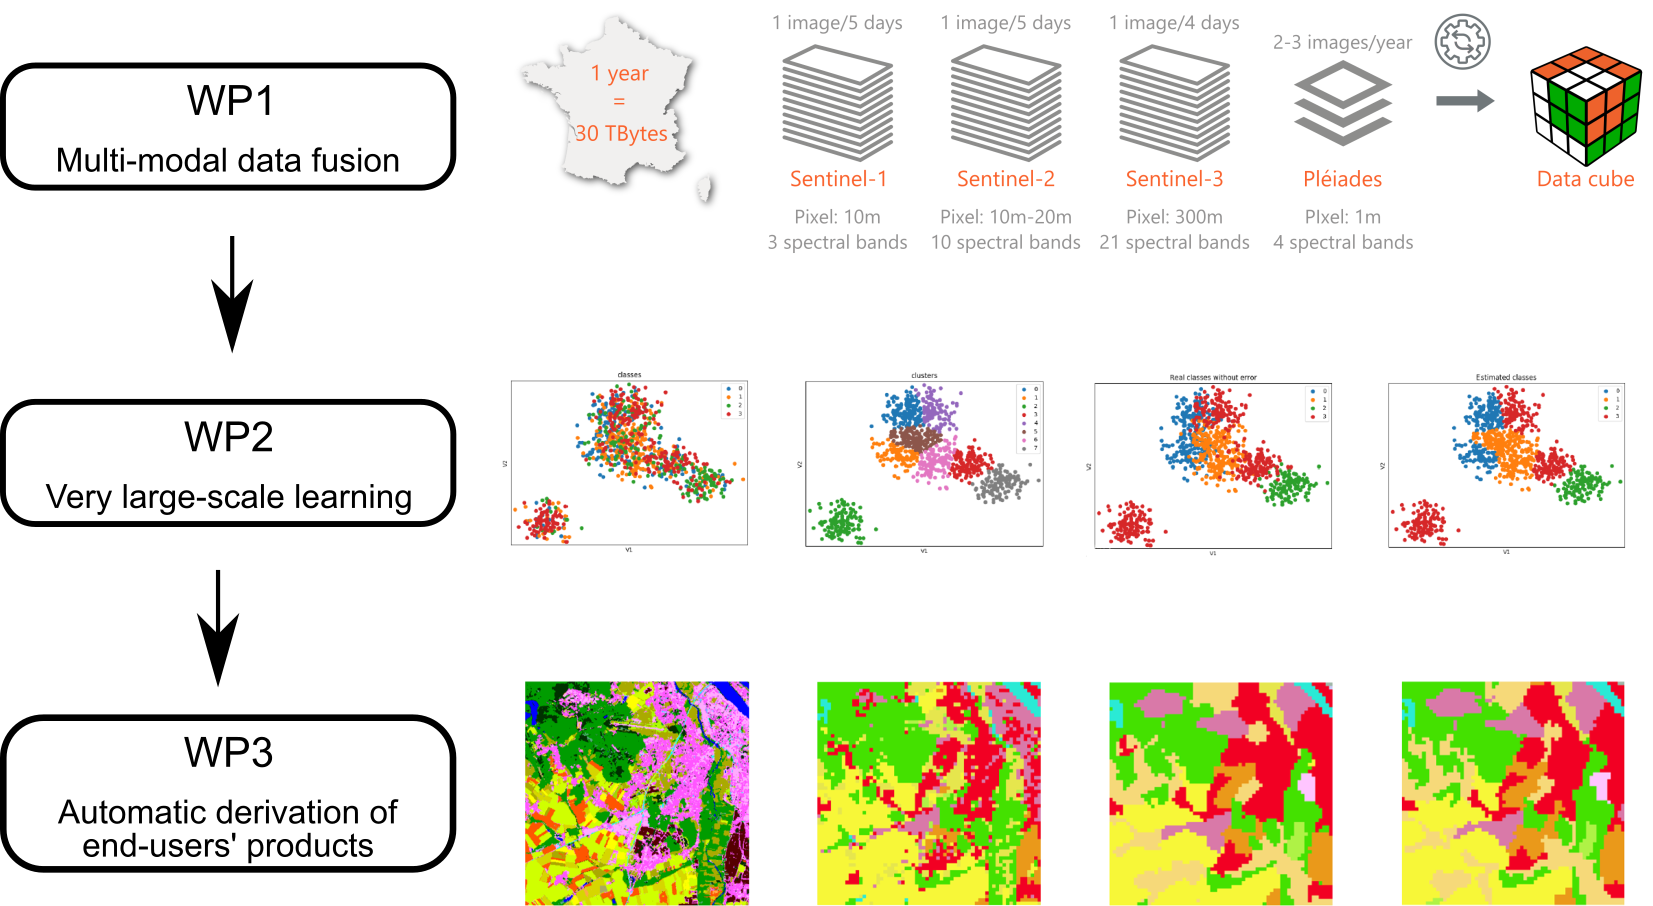
\includegraphics[width=0.9\columnwidth]{img/wp_maestria.png}
    \caption{Architecture of the MAESTRIA project. From raw EO data to on-purpose land-cover maps.}
    \label{fig:enter-label}
\end{figure}



\subsubsection*{Informations factuelles}

Le projet ANR MAESTRIA est un projet de recherche fondamentale coordonné par Clément Mallet (LASTIG) conjointement avec le CESBIO. Le projet a commencé en octobre 2019 et a duré 54 mois. Il a bénéficié d’une aide ANR de 568$\:$k€ pour un coût global de l’ordre de \textcolor{red}{??}$\:$k€. Il a reçu le soutien du pôle de compétitivité Aerospace Valley.


\subsection{Résumé consolidé public en anglais}

Transposition en anglais (deepL quoi\ldots)